\documentclass{article}
\usepackage[T1,T2A]{fontenc}
\usepackage[utf8x]{inputenc}
\usepackage[10pt]{extsizes}
\usepackage{geometry}
\usepackage{xcolor}
\usepackage{tikz}
\usepackage{graphicx, caption}
\usepackage{wrapfig}
\usepackage{amssymb}

\geometry{top=4em,right=3em,left=3em,bottom=4em}

\begin{document}
\newcommand{\Mainclt}{\raisebox{0pt}[\headheight][30pt]{\vbox{\hbox to\textwidth{48\hfilКНИГА I ПРЕДЛ. XXIV. ТЕОРЕМА\hfil}}}}
\begin{minipage}[t]{0.4\textwidth}
  \hfill \\
  \begin{center}
    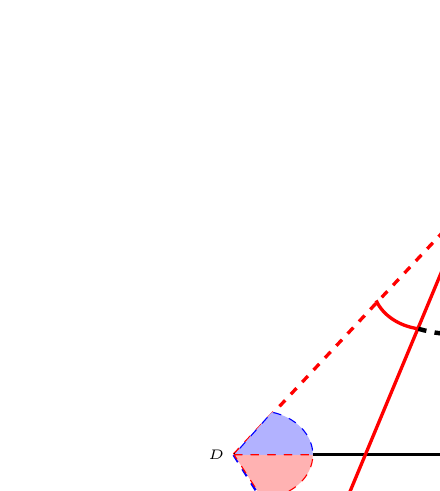
\begin{tikzpicture}[xscale=1.0, yscale=0.8]
      \draw[dashed,red,very thick] (0,0) -- (3,4);
      \draw[very thick] (0,0) -- (4,0);
      \draw[red,very thick] (1,-2) -- (3,4);
      \draw[blue,very thick] (3,4) -- (4,0);
      \draw[dashed,very thick] (1,-2) -- (4,0);
      \draw[dashed,blue,very thick] (0,0) -- (1,-2);
      \node[left] at (0,0) {{\tiny$D$}};
      \node[right] at (4,0) {{\tiny$B$}};
      \node[below] at (1,-2) {{\tiny$C$}};
      \node[above] at (3,4) {{\tiny$A$}};
      \draw[dashed,blue,fill=blue!30] (0,0) --  (0:1) arc(0:75:0.7) -- cycle;
      \draw[dashed,red,fill=red!30] (0,0) --  (0:1) arc(0:-85:0.7) -- cycle;
      \draw[dashed,yellow,fill=orange!70] (1,-2) -- (1.3,-1) arc(40:140:0.5) -- cycle;
      \draw[dashed,black,fill=black!70] (1,-2) -- (1.7,-1.6) arc(40:86:0.7) -- cycle;
      \draw[red,very thick] (2.34,2) arc(260:200:0.7);
      \draw[dashed,ultra thick] (2.34,2) arc(250:295:1.5);
    \end{tikzpicture}
    \begin{tikzpicture}[xscale=1.0, yscale=0.8]
      \draw[orange,very thick] (1,-2) -- (4,0);
      \draw[blue,very thick] (3,4) -- (4,0);
      \draw[red,very thick] (1,-2) -- (3,4);
      \node[right] at (4,0) {{\tiny$F$}};
      \node[below] at (1,-2) {{\tiny$G$}};
      \node[above] at (3,4) {{\tiny$E$}};
      \draw[dashed,ultra thick] (2.34,2) arc(250:295:1.5);
    \end{tikzpicture}
  \end{center}
\end{minipage}
\hfil
\begin{minipage}[t]{0.55\textwidth}
  \Mainclt
  \begin{wrapfigure}{l}{0.2\linewidth}
    
\includegraphics[width=0.9\linewidth]{src/E.jpg}
  \end{wrapfigure}\\
  \slshape сли у двух треугольников по две стороны соответсвенно равны друг другу (
  \begin{tikzpicture}
    \draw[blue,very thick] (0,0) -- (1,0);
    \node[above] at (0,0) {{\tiny$A$}};
    \node[above] at (1,0) {{\tiny$B$}};
  \end{tikzpicture} =
  \begin{tikzpicture}
    \draw[blue,very thick] (0,0) -- (1,0);
    \node[above] at (0,0) {{\tiny$E$}};
    \node[above] at (1,0) {{\tiny$F$}};
  \end{tikzpicture} и 
  \begin{tikzpicture}
    \draw[dashed,orange,very thick] (0,0) -- (1,0);
    \node[above] at (0,0) {{\tiny$A$}};
    \node[above] at (1,0) {{\tiny$D$}};
  \end{tikzpicture} =
  \begin{tikzpicture}
    \draw[orange,very thick] (0,0) -- (1,0);
    \node[above] at (0,0) {{\tiny$G$}};
    \node[above] at (1,0) {{\tiny$E$}};
  \end{tikzpicture}), и угол заключенный междуними в одном
  \begin{tikzpicture}
    \draw[dashed,red,ultra thick] (0,0) -- (0.5,0.3);
    \draw[red,ultra thick] (0.35,-0.2) -- (0.5,0.3);
    \draw[blue,ultra thick] (0.75,-0.22) -- (0.5,0.3);
    \draw[red,ultra thick] (0,0) arc (220:265:0.5);
    \draw[dashed,ultra thick] (0.4,-0.2) arc (250:295:0.5);
    \node[above] at (0.5,0.3) {{\tiny$A$}};
    \node[left] at (0,0) {{\tiny$D$}};
    \node[right] at (0.75,-0.22) {{\tiny$B$}};
  \end{tikzpicture}
  больше, чем в другом
  \begin{tikzpicture}
    \draw[red,ultra thick] (0.35,-0.2) -- (0.5,0.3);
    \draw[blue,ultra thick] (0.75,-0.22) -- (0.5,0.3);
    \draw[dashed,ultra thick] (0.4,-0.2) arc (250:295:0.5);
    \node[above] at (0.5,0.3) {{\tiny$E$}};
    \node[below] at (0.75,-0.22) {{\tiny$F$}};
    \node[below] at (0.35,-0.2) {{\tiny$G$}};
  \end{tikzpicture}, то сторона
  \begin{tikzpicture}
    \draw[very thick] (0,0) -- (1,0);
    \node[above] at (0,0) {{\tiny$D$}};
    \node[above] at (1,0) {{\tiny$B$}};
  \end{tikzpicture}противолежащая большему углу больше стороны, противолежащей меньшему
  \begin{tikzpicture}
    \draw[yellow,very thick] (0,0) -- (1,0);
    \node[above] at (0,0) {{\tiny$F$}};
    \node[above] at (1,0) {{\tiny$G$}};
  \end{tikzpicture}.
  \upshape
  \begin{center}
    Сделаем
    \begin{tikzpicture}
      \draw[red,ultra thick] (0.35,-0.2) -- (0.5,0.3);
      \draw[blue,ultra thick] (0.75,-0.22) -- (0.5,0.3);
      \draw[dashed,ultra thick] (0.4,-0.2) arc (250:295:0.5);
      \node[above] at (0.5,0.3) {{\tiny$A$}};
      \node[below] at (0.75,-0.22) {{\tiny$B$}};
      \node[below] at (0.35,-0.2) {{\tiny$C$}};
    \end{tikzpicture}=
    \begin{tikzpicture}
      \draw[red,ultra thick] (0.35,-0.2) -- (0.5,0.3);
      \draw[blue,ultra thick] (0.75,-0.22) -- (0.5,0.3);
      \draw[dashed,ultra thick] (0.4,-0.2) arc (250:295:0.5);
      \node[above] at (0.5,0.3) {{\tiny$E$}};
      \node[below] at (0.75,-0.22) {{\tiny$F$}};
      \node[below] at (0.35,-0.2) {{\tiny$G$}};
    \end{tikzpicture} (пр. I.{\tiny23}),\\
    и
    \begin{tikzpicture}
      \draw[red,very thick] (0,0) -- (1,0);
      \node[above] at (0,0) {{\tiny$C$}};
      \node[above] at (1,0) {{\tiny$A$}};
    \end{tikzpicture} =
    \begin{tikzpicture}
      \draw[orange,very thick] (0,0) -- (1,0);
      \node[above] at (0,0) {{\tiny$G$}};
      \node[above] at (1,0) {{\tiny$E$}};
    \end{tikzpicture} (пр. I.{\tiny3}),\\
    проведем
    \begin{tikzpicture}
      \draw[dashed,blue,very thick] (0,0) -- (1,0);
      \node[above] at (0,0) {{\tiny$C$}};
      \node[above] at (1,0) {{\tiny$D$}};
    \end{tikzpicture} и
    \begin{tikzpicture}
      \draw[dashed,very thick] (0,0) -- (1,0);
      \node[above] at (0,0) {{\tiny$B$}};
      \node[above] at (1,0) {{\tiny$C$}};
    \end{tikzpicture}.\\
    \vspace{0.4cm}
    Поскольку
    \begin{tikzpicture}
      \draw[orange,very thick] (0,0) -- (1,0);
      \node[above] at (0,0) {{\tiny$C$}};
      \node[above] at (1,0) {{\tiny$A$}};
    \end{tikzpicture}=
    \begin{tikzpicture}
      \draw[orange,dashed,very thick] (0,0) -- (1,0);
      \node[above] at (0,0) {{\tiny$A$}};
      \node[above] at (1,0) {{\tiny$D$}};
    \end{tikzpicture} (акс. I, гип., постр.)\\
    $\therefore$
    \begin{tikzpicture}
      \draw[dashed,blue,fill=blue!30] (0,0) --  (1,0) arc(0:75:0.7) -- cycle;
      \draw[dashed,red,fill=red!30] (0,0) --  (1,0) arc(0:-85:0.7) -- cycle;
      \node[below] at (0.65,1) {{\tiny$A$}};
      \node[left] at (0,0) {{\tiny$D$}};
      \node[right] at (0.35,-0.75) {{\tiny$C$}};
    \end{tikzpicture} = 
    \begin{tikzpicture}
      \draw[dashed,yellow,fill=orange!70] (1,-2) -- (1.3,-1) arc(40:140:0.5) -- cycle;
      \node[right] at (1.2,-1) {{\tiny$A$}};
      \node[left] at (0.65,-1) {{\tiny$D$}};
      \node[below] at (1,-2) {{\tiny$C$}};
    \end{tikzpicture} (пр. I.{\tiny 5}), но
    \begin{tikzpicture}
      \draw[dashed,red,fill=red!30] (0,0) --  (1,0) arc(0:-85:0.7) -- cycle;
      \node[left] at (0,0) {{\tiny$D$}};
      \node[right] at (1,0) {{\tiny$B$}};
      \node[left] at (0.65,-1) {{\tiny$C$}};
    \end{tikzpicture} $<$
    \begin{tikzpicture}
      \draw[dashed,yellow,fill=orange!70] (1,-2) -- (1.3,-1) arc(40:140:0.5) -- cycle;
      \node[below] at (1,-2) {{\tiny$C$}};
      \node[right] at (1.2,-1) {{\tiny$A$}};
      \node[left] at (0.65,-1) {{\tiny$D$}};
    \end{tikzpicture},\\
    и $\therefore$
    \begin{tikzpicture}
      \draw[dashed,red,fill=red!30] (0,0) --  (1,0) arc(0:-85:0.7) -- cycle;
      \node[left] at (0,0) {{\tiny$D$}};
      \node[right] at (1,0) {{\tiny$B$}};
      \node[left] at (0.65,-1) {{\tiny$C$}};
    \end{tikzpicture} $<$
    \begin{tikzpicture}
      \draw[dashed,yellow,fill=orange!70] (1,-2) -- (1.3,-1) arc(40:140:0.5) -- cycle;
      \draw[dashed,black,fill=black!70] (1,-2) -- (1.7,-1.6) arc(40:86:0.7) -- cycle;
      \node[below] at (1,-2) {{\tiny$C$}};
      \node[right] at (1.6,-1.6) {{\tiny$B$}};
      \node[left] at (0.65,-1) {{\tiny$D$}};
    \end{tikzpicture},\\
    \vspace{0.4cm}
    $\therefore$
    \begin{tikzpicture}
      \draw[very thick] (0,0) -- (1,0);
      \node[above] at (0,0) {{\tiny$D$}};
      \node[above] at (1,0) {{\tiny$B$}};
    \end{tikzpicture} $>$ 
    \begin{tikzpicture}
      \draw[dashed,very thick] (0,0) -- (1,0);
      \node[above] at (0,0) {{\tiny$B$}};
      \node[above] at (1,0) {{\tiny$C$}};
    \end{tikzpicture} (пр. I.{\tiny 19})\\
    \vspace{0.4cm}
    но
    \begin{tikzpicture}
      \draw[dashed,very thick] (0,0) -- (1,0);
      \node[above] at (0,0) {{\tiny$B$}};
      \node[above] at (1,0) {{\tiny$C$}};
    \end{tikzpicture} $=$
    \begin{tikzpicture}
      \draw[yellow,very thick] (0,0) -- (1,0);
      \node[above] at (0,0) {{\tiny$F$}};
      \node[above] at (1,0) {{\tiny$G$}};
    \end{tikzpicture} (пр. I.{\tiny 4})\\
    \vspace{0.4cm}
    $\therefore$
    \begin{tikzpicture}
      \draw[very thick] (0,0) -- (1,0);
      \node[above] at (0,0) {{\tiny$D$}};
      \node[above] at (1,0) {{\tiny$B$}};
    \end{tikzpicture} $>$
    \begin{tikzpicture}
      \draw[yellow,very thick] (0,0) -- (1,0);
      \node[above] at (0,0) {{\tiny$F$}};
      \node[above] at (1,0) {{\tiny$G$}};
    \end{tikzpicture}
  \end{center}
  \begin{flushright}
    ч. т. д.
  \end{flushright}
\end{minipage}
\end{document}